\documentclass[12pt,twoside]{rif}

\pagestyle{myheadings}
\usepackage[
left=2.54cm,
right=2.54cm,
top=2.54cm,
bottom=2.54cm]
{geometry}
\usepackage{hyperref}
\usepackage{natbib}
\usepackage{subfigure}
\hypersetup{
	urlcolor=blue, 
	colorlinks=true, 
	citecolor=blue
}

\usepackage{lipsum}

\title{\textbf{Dilatación del tiempo gravitacional}}

\author[1]{{\small Carlos Andrés García Suarez}} 
\author[1]{{\small David Brandon Zevallos Garay}}
\author[1]{{\small Luis Fernando Ubillus Benites}}
%\author[3]{Autor3}
\affil[1]{{ \small Facultad de Ciencias Naturales y Matemática, Universidad
		Nacional Federico Villarreal. El Agustino 15003. Lima-Perú.}}
%\affil[2,3]{Afiliacion2}
%\date{\normalsize Recibido: xxxx Aceptado: xxxx Publicado: xxxx\\
%Todos los derechos reservados-SEF \copyright{} 2012}
\date{}

\begin{document}
	\maketitle
	
	\begin{res}
		\begin{center}
			\textbf{Resumen} \\
		\end{center}
		\lipsum[2]
		
		\par
		\smallskip
		\clav{sdjssasdfsdf, asdfsdf, asdfsdafsd}
	\end{res}
	\begin{center}
		\title{\textbf{Time gravitational dilation}}
	\end{center}
	
	\begin{abst}
		\begin{center}
			\textbf{Abstract} \\
		\end{center}
		\lipsum[2]
		
		\par 
		\smallskip
		\key{sdjssasdfsdf, asdfsdf, asdfsdafsd}
	\end{abst}

	
	
	\newpage
	
	\tableofcontents
	
	\section{ Introducción} 
	
	\section{Marco Teórico}
	\subsection{Teoria de la Relatividad Especial}
	Este es el enfoque moderno que le dio Albert Einsten a la fisica, donde se "olvida" el concepto de tiempo y distancia Absoluto de la Teoria de Newton.
	Esta teoria se basa en dos postulados simplemente:
	Las leyes de la Fisica son validas para todos los sistemas "inerciales"
	 La velocidad de la luz en el vacio es igual para todos los observadores 
	Hay que tener cuidado con la palabra inercial que es su campo de aplicacion.
	\subsection{Principio de equivalencia}
	Un punto clave en este trabajo es el principio de equivalencia, que nos dice que un observador en caida libre en un campo gravitatorio es equivalente a un observador en el espacio fuera de toda influencia gravitatoria. Todo esto de forma local hasta que este sienta las consecuencias de la curvatura. Pero tambien nos dicen que un observador acelerado con aceleracion a en el espacio sin influencia de gravedad,es equivalente a un observador inercial en tierra con una gravedad igual a -a. Todo esto de forma local, hasta que el observador en el espacio se de cuenta que no sigue una geodesica.
	\subsection{Principio de Covariancia}
	"Este principio nos indica que el lenguaje tensorial permite escribir las leyes de la Fisica de manera que son validas para todos los observadores." (Expo2,pag 151)
	\subsection{Sistema Inecial}
	Dado que para Newton un Sistema inercial es aquel que tiene una velocidad relativa a otro en reposo, para este estaba bien definido este concepto, pero gracias al principio de equivalencia se observa que un observador acelerado tambien se puede considerar a si mismo como inercial por lo menos de forma local...
	\section{Conclusiones}
\begin{center}
\begin{figure}
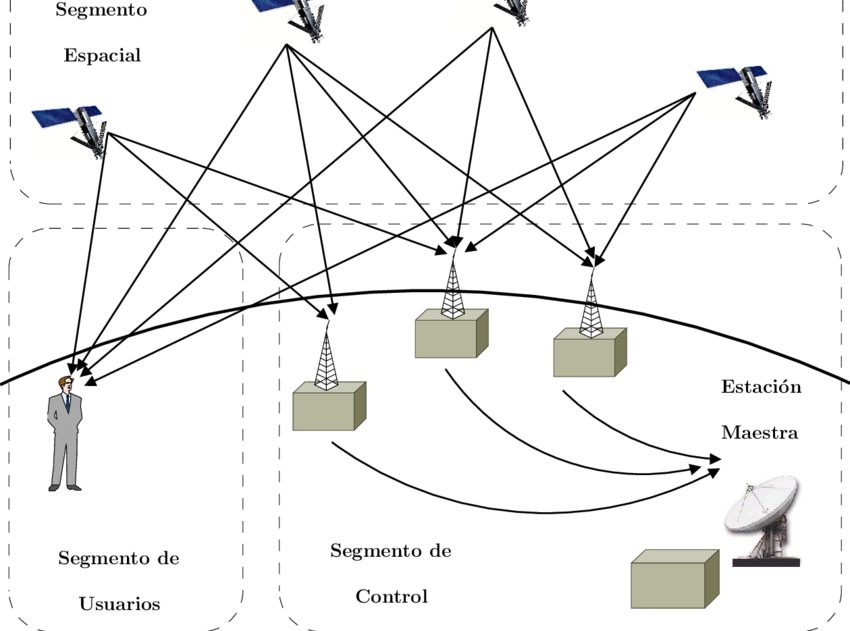
\includegraphics[width=0.8\textwidth]{img/GPS.png}
\end{figure}
\end{center}
	\nocite{*}
	\bibliographystyle{apa}
	\bibliography{biblio}
	

\end{document}